\documentclass[12pt]{article}

\usepackage[letterpaper]{geometry}
\usepackage{color}
\usepackage{listings}
\usepackage{natbib}
\usepackage{graphicx}

\graphicspath{{figs/}}

\definecolor{beige}{RGB}{245,245,220}

\newcommand{\jlt}[1]{\textcolor{red}{(#1)}}

\newcommand{\braidlab}{\texttt{braidlab}}%{\lstinline{braidlab}}
\newcommand{\braid}{\texttt{braid}}%{\lstinline{braid}}
\newcommand{\loopc}{\texttt{loop}}%{\lstinline{loop}}

\begin{document}

\lstset{language=Matlab}
\lstset{breaklines=true}
\lstset{backgroundcolor=\color{beige}}
%\lstset{emph={directory,containing,{+}braidlab},emphstyle=\color{red}}

\lstset{% general command to set parameter(s)
basicstyle=\small\ttfamily,
keywordstyle=\small\ttfamily,
identifierstyle=,
commentstyle=\small\ttfamily,
stringstyle=\small\ttfamily,
showstringspaces=false}


\title{\braidlab\ user's guide}
\author{Jean-Luc Thiffeault}
\maketitle

\section{Installing \braidlab}

The package \braidlab\ is defined inside a Matlab namespace, which are
specified as subfolders beginning with a `+' character.  The Matlab
path must contain the folder that contains the subfolder
\lstinline{+braidlab}, and not the \lstinline{+braidlab} folder
itself:
\begin{lstlisting}[frame=single,framerule=0pt]
>> addpath <folder containing +braidlab>
\end{lstlisting}
Then, to execute a braidlab function, either call it using the syntax
\lstinline{braidlab.<function>}, or import the whole namespace:
\begin{lstlisting}[frame=single,framerule=0pt]
>> import braidlab.*
\end{lstlisting}
This allows execution of \lstinline{<function>} by itself, without the
\lstinline{braidlab} prefix.  For the remainder of this document, we
assume this has been done and omit the \lstinline{braidlab} prefix.

\section{A tour of \braidlab}

\subsection{The \braid\ class}

\braidlab\ defines a number of classes, most importantly \braid\ and
\loopc.  The braid~$\sigma_1\sigma_2^{-1}$ is defined by
\begin{lstlisting}[frame=single,framerule=0pt]
>> a = braid([1 -2])

a = < 1 -2 >
\end{lstlisting}
which defaults to the minimum required strands,~$3$.  To same braid
on~$4$ strands is defined by
\begin{lstlisting}[frame=single,framerule=0pt]
> a4 = braid([1 -2],4)

a4 = < 1 -2 >
\end{lstlisting}
Two braids can be multiplied:
\begin{lstlisting}[frame=single,framerule=0pt]
>> a = braid([1 -2]); b = braid([1 2]);
>> a*b, b*a

ans = < 1 -2  1  2 >

ans = < 1  2  1 -2 >
\end{lstlisting}
Powers can also be taken, including the inverse:
\begin{lstlisting}[frame=single,framerule=0pt]
>> a^5, inv(a), a*a^-1

ans = < 1 -2  1 -2  1 -2  1 -2  1 -2 >

ans = <2 -1>

ans = < 1 -2  2 -1 >
\end{lstlisting}
Note that this last expression is the identity braid, but is not
simplified.  The method \lstinline{compact} attempts to simplify the
braid:
\begin{lstlisting}[frame=single,framerule=0pt]
>> compact(a*a^-1)

ans = < e >
\end{lstlisting}
The method \lstinline{compact} is based on the heuristic algorithm
of~\cite{Bangert2002}, since finding the braid of minimum length in
the standard generators is in general difficult~\citep{Paterson1991}.

The number of strings is
\begin{lstlisting}[frame=single,framerule=0pt]
>> a.n

ans = 3
\end{lstlisting}
Note that
\begin{lstlisting}[frame=single,framerule=0pt]
>> help braid
\end{lstlisting}
describes the class \braid.  To get more information on the \braid\
constructor, invoke
\begin{lstlisting}[frame=single,framerule=0pt]
>> help braid.braid
\end{lstlisting}
which refers to a method within the class \braid.  There are other
ways to construct a \braid, such as using random generators, here a
braid with~$5$ strings and~$10$ random generators:
\begin{lstlisting}[frame=single,framerule=0pt]
>> braid('random',5,10)

ans = < 1  4 -4  2  4 -1 -2  4  4  4 >
\end{lstlisting}
The constructor can also build some standard braids:
\begin{lstlisting}[frame=single,framerule=0pt]
>> braid('halftwist',5)

ans = < 4  3  2  1  4  3  2  4  3  4 >
\end{lstlisting}
In Section~\ref{sec:braidfromdata} we will also show how to construct
a braid from a trajectory data set.

The \braid\ class also handles equality of braids:
\begin{lstlisting}[frame=single,framerule=0pt]
>> a = braid([1 -2]); b = braid([1 -2 2 1 2 -1 -2 -1]);
>> a == b

ans = 1
\end{lstlisting}
These are the same braid.  Equality is determined efficiently by
acting on loop (Dynnikov) coordinates~\citep{Dynnikov2002}, as
described by \citet{Dehornoy2008}.

We can extract a subbraid by choosing specific strings: for example,
if we take the~$4$-string braid~$\sigma_1\sigma_2\sigma_3^{-1}$ and
discard the third string, we obtain~$\sigma_1\sigma_2^{-1}$:
\begin{lstlisting}[frame=single,framerule=0pt]
>> a = braid([1 2 -3]);
>> subbraid(a,[1 2 4])

ans = < 1 -2 >
\end{lstlisting}

There are a few methods that exploit the connection between braids and
homeomorphisms of the punctured disk.  Braids label \emph{isotopy
  classes} of homeomorphisms, so we can assign a topological entropy
to a braid:
\begin{lstlisting}[frame=single,framerule=0pt]
>> entropy(braid([1 2 -3]))

ans = 0.8314
\end{lstlisting}
The entropy is computed by iterated action on a
loop~\citep{Moussafir2006}.  This can fail if the braid is
finite-order or has very low entropy:
\begin{lstlisting}[frame=single,framerule=0pt]
>> entropy(braid([1 2]))
Warning: Failed to converge to requested tolerance; braid is likely finite-order or has low entropy. 
> In braid.entropy at 89

ans = 0
\end{lstlisting}

To force the entropy to be computed using
the Bestvina--Handel train track algorithm~\cite{Bestvina1995}, we add
a flag:
\begin{lstlisting}[frame=single,framerule=0pt]
>> entropy(braid([1 2]),'trains')

ans = 0
\end{lstlisting}
Note that for large braids the Bestvina--Handel algorithm is
impractical.  But when it can be used it can also determine the
Thurton--Nielsen type of the
braid~\citep{Fathi1979,Thurston1988,Casson1988,Boyland1994}:
\begin{lstlisting}[frame=single,framerule=0pt]
>> tntype(braid([1 2 -3]))

ans = pseudo-Anosov
>> tntype(braid([1 2]))

ans = finite-order
>> tntype(braid([1 2],4))

ans = reducible
\end{lstlisting}
\braidlab\ uses Toby Hall's implementation of the Bestvina--Handel
algorithm~\citep{HallTrain}.

Finally, we can also find the Burau
representation~\citep{Burau1936,Birman1975} of a braid:
\begin{lstlisting}[frame=single,framerule=0pt]
>> burau(braid([1 -2]),-1)

ans = 1    -1
     -1     2
\end{lstlisting}
where the last argument ($-1$) is the value of the parameter~$t$ in
the Laurent polynomials that appear in the entries of the Burau
matrices.


\subsection{Constructing a braid from data}
\label{sec:braidfromdata}

One of the main purposes of \braidlab\ is to analyze two-dimensional
trajectory data using braids.  The folder \lstinline{testing} contains
a dataset of trajectories, from laboratory data for granular
media~\cite{Puckett2012}.  Figure~\ref{fig:testdata_trajs} shows
%
\begin{figure}
\begin{center}
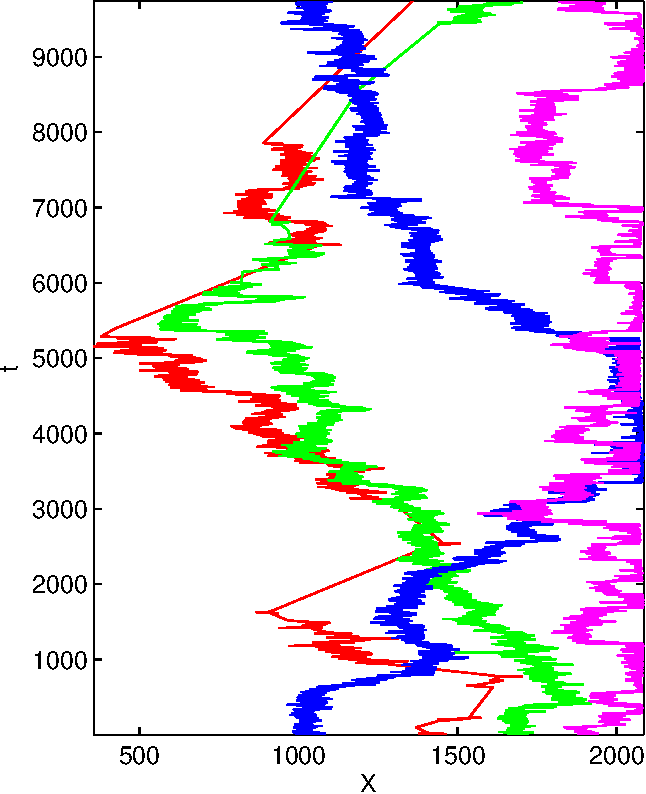
\includegraphics[width=.5\textwidth]{testdata_trajs}
\end{center}
\caption{}
\label{fig:testdata_trajs}
\end{figure}
%
the~$X$ coordinate of these four trajectories, with time plotted
vertically.  From the \lstinline{testing} folder, we load the data:
\begin{lstlisting}[frame=single,framerule=0pt]
>> clear; load testdata
>> whos
  Name         Size               Bytes  Class     Attributes

  XY        9740x2x4             623360  double              
  ti           1x9740             77920  double              
\end{lstlisting}
Here \lstinline{ti} is the vector of times, and \lstinline{XY} is a
three-dimensional array: its first component specifies the timestep,
its second specifies the $X$ or $Y$ coordinate, and its third
specifies one of the~$4$ particles.  To construct a braid from this
data, we simply execute
\begin{lstlisting}[frame=single,framerule=0pt]
>> b = braid(XY);
>> b.length

ans = 896
\end{lstlisting}
This is a very long braid!  But Figure~\ref{fig:testdata_trajs}
suggests that this is perhaps misleading: many of the crossings are
`wiggles' that cancel each other out.  Indeed, if we attempt to
shorten the braid:
\begin{lstlisting}[frame=single,framerule=0pt]
>> b = compact(b)

b = < -1 -2 -1 -1 -1 -1 -1 -1 -1 -1 -1  3  1  3  2  1 >
>> b.length

ans = 16
\end{lstlisting}
\jlt{This could be shorter! Why is $-1,3,1$ not getting simplified to
  $3$?}  we find the number of generators (the length) has dropped
to~$16$!

\jlt{Discuss closure?}

% \lstinputlisting[lastline=50]{+braidlab/@braid/braid.m}

\bibliographystyle{jfm}
\bibliography{braidlab_guide}

\end{document}
